\section{Experimental Setup}
\label{sec:experiments}

\subsection{Benchmark Design}

We build the cross-material benchmark in the Genesis multi-physics simulator~\cite{genesis2024} around a single \emph{edge-push} task. A Franka Panda arm (7 DoF) equipped with a flat scoop end-effector must push a pile of particles from an elevated source platform across a raised edge into a target bin, with spill onto the floor penalized. This task is deliberately simple kinematically---it is essentially a horizontal push followed by a settle---which reduces, but does not eliminate, task-engineering confounds when comparing material-regime behavior.

\cref{fig:scene_schematic} shows the fixed edge-push scene, and Appendix \cref{tab:benchmark} reports the split parameters. The same Franka, scoop, source platform, target bin, and pile placement (Config D, 5.5\,cm from the open edge) are used for every split, so cross-split differences come from material parameters alone. We use Genesis MPM at grid density 128 with 25 substeps per control step (control $\Delta t = 2 \times 10^{-3}$~s).

\begin{figure}[t]
    \centering
    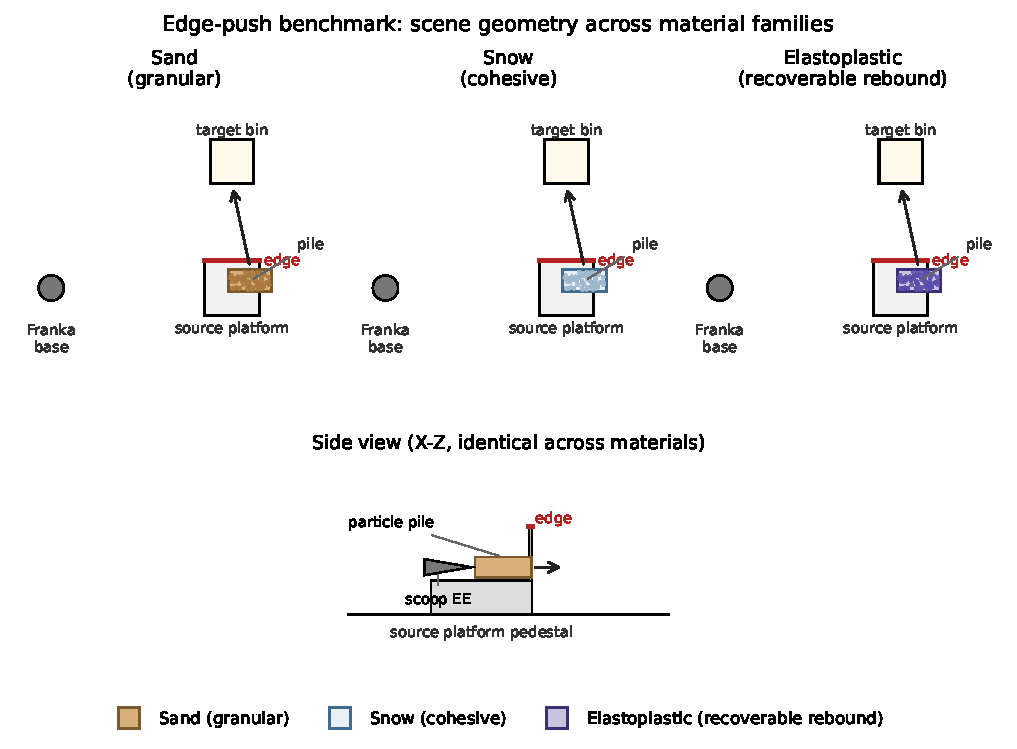
\includegraphics[width=0.88\textwidth]{figures/fig5_scene_schematic.pdf}
    \caption{\textbf{Genesis edge-push benchmark.} Representative settled-pile renders; geometry is fixed across panels, while MPM material parameters and scripted-transfer difficulty differ.}
    \label{fig:scene_schematic}
\end{figure}

\paragraph{Material choices.}
The three material families span clean and boundary regimes. \emph{Sand} (granular, $E=5 \times 10^4$, $\nu=0.3$, $\rho=2000$) is the training material and the hardest---a scripted baseline achieves only 32\% transfer because particles deform under the scoop and flow backward. \emph{Elastoplastic} ($E=5 \times 10^4$, $\nu=0.4$, $\rho=1000$) is the clean recoverable case: the pile partially rebounds after each push, so a fixed residual over-corrects. \emph{Snow} (cohesive, $E=1 \times 10^5$, $\nu=0.2$, $\rho=400$) is deliberately a boundary case. Cohesion makes the scripted push easy (87\% transfer), but contact loading can leave a compacted or displaced region rather than a rebounded one, so recoverability is not equated with cohesion or task ease. We use ``elastoplastic'' throughout to refer to this Genesis material model and reserve ``viscoelastic'' as a description of the rebound behavior it exhibits, rather than as an independent material class. The 55pp spread between hardest and easiest is \emph{discriminative} by design, making a single push profile insufficient for uniformly high scripted transfer.

\paragraph{OOD parameter splits.}
In addition to family-level OOD (snow, elastoplastic), we evaluate on parameter-shifted sand variants: \textbf{Sand-Hard} ($E=8 \times 10^4$, 60\% stiffer) and \textbf{Sand-Soft} ($E=2 \times 10^4$, 60\% softer). These probe within-family generalization and serve as controls: if a method's gain on elastoplastic is driven by generic ``any-OOD'' robustness, the parameter splits should show similar gains.

\subsection{Evaluation Protocol}

All methods train on ID sand only and are evaluated zero-shot on the four other splits, testing \emph{extrapolation} rather than interpolation over a labeled material mix. Each (method, seed, split) is scored by 10 deterministic-policy episodes. Metrics: (i) transfer efficiency (fraction of particles delivered to the target), (ii) spill ratio (fraction off the platform/outside the target), and (iii) success rate (fraction of episodes exceeding 30\% transfer; the 30\% threshold is a level the scripted controller exceeds on snow and elastoplastic but not on sand, distinguishing bulk delivery from stirring). M1, M7, and the M7 ablations use three seeds (42, 0, 1) and report mean $\pm$ std; M8 is scored as a single-seed diagnostic baseline. NaN rollouts (rare, from Genesis contact blowups) count as zero-transfer/unit-spill failures so a method cannot benefit from crashing the simulator.

\subsection{Compared Systems}

We compare five systems, all trained with identical 500\,k-step PPO budgets and matched hyperparameters (residual scale 0.05, observation: proprio + particle statistics):

\begin{itemize}
    \item \textbf{M1: Reactive PPO}---standard reactive baseline conditioned on $s_t$ only. No probe, no belief.
    \item \textbf{M7: \PTA{} (ours)}---the full two-stage architecture of \cref{sec:method}.
    \item \textbf{M8: Privileged-Parameter Baseline}---a sand-only-trained residual policy that additionally receives ground-truth material parameters (7-D privileged observation) concatenated to $s_t$, but is otherwise matched to M1/M7. It tests parameter access under the same sand-only training protocol.
    \item \textbf{M7-NoProbe}---ablation that skips the probing phase; encoder sees a zero trace.
    \item \textbf{M7-NoBelief}---ablation that runs the probe but drops the encoder output.
\end{itemize}

M1 and M7 are the core comparison. M8 is a privileged \emph{controlled} baseline---matched architecture and training protocol, plus ground-truth parameters---so it isolates the value of those parameters under sand-only training rather than serving as a universal informational upper bound. The two ablations localize \PTA{}'s gain across its components.

\subsection{Implementation Details}

All runs use PPO from Stable-Baselines3~\cite{raffin2021stable} with MLP policy/value heads of size $[256,256]$, lr $3\times10^{-4}$, batch 64, 10 epochs/update, $\gamma=0.99$. The 7-DoF residual is added to a 410-step scripted edge-push trajectory followed by an 80-step settle; joint targets are commanded via \texttt{set\_qpos}, which in our environment bypasses single-step DLS-IK coupling artifacts. Code, configurations, and seeds will be released upon acceptance.
